% high IPC realization
%
%\documentclass[10pt,twocolumn,dvips]{article}
\documentclass[10pt,dvips]{article}
\usepackage[english]{babel}
\usepackage{epsfig}
%
%\usepackage{fancyheadings}
%\usepackage[T1]{fontenc}
%\usepackage[latin1]{inputenc}
%
%\usepackage{twocolumn}
%\usepackage{verbatim,moreverb,doublespace}
%\usepackage{rotate,lscape,dcolumn,array,rotating,latexsym}
%
%\input{epsf}
%
\textwidth 6.5in
\textheight 9.0in
\topmargin -0.6in
\oddsidemargin 0mm
\evensidemargin 0mm
%
\pagestyle{empty}
%
\begin{document}
\parskip 3mm
%
%
\title{Realizing High IPC Through a Large Microarchitecture}
%
\author{
A. Khalafi, D. Morano, D.R. Kaeli\\
Northeastern University\\
{akhalafi, dmorano, kaeli}@ece.neu.edu\\
\and
A.K. Uht \\
University of Rhode Island\\ uht@ele.uri.edu
}
%
\maketitle
\thispagestyle{empty}
%
\begin{abstract}
This paper explores a microarchitecture that achieves high execution
performance on conventional single-threaded program codes without
compiler assistance.  Larger microarchitectures can have several
hundreds of speculative instructions in-flight simultaneously.  This
provides a means to extract larger amounts of instruction level
parallelism even from programs that are very sequential in nature.
However, several problems are associated with a large
microarchitecture.  Among these are scalability issues, speculative
control flow issues, and the memory latency problem.

We present a basic overview of our microarchitecture and how it
addresses the problem of scalability.  We also discuss how we use
multipath execution to try and address the problem of mispredicted
conditional branches.  We provide simulation results for several
configurations of our microarchitecture that illustrate how higher IPC
can be realized from serial-oriented integer programs.  We also present
data that shows the positive effects of applying multipath execution to
the same programs.  Finally, we present data that shows our
microarchitecture's tolerance of high memory latency.
\end{abstract}
%
\section{Introduction}
%
A number of studies into the limits of instruction level 
parallelism (ILP) have
been promising in that they have shown that there is 
a significant amount of parallelism within
typical sequentially oriented single-threaded programs
(e.g., SpecInt-2000).  
The work of researchers like
Lam and Wilson ~\cite{Lam92},
Uht and Sindagi ~\cite{Uht95},
Gonzalez and Gonzalez ~\cite{Gon97}
have shown that there exists a great amount of instruction level
parallelism (ILP) that is not being exploited by any existing
computer designs.
Unfortunately, most of the fine-grained instruction level
parallelism inherent in integer sequential programs
spans several basic blocks.  
Data and control independent instructions, that may exist
far ahead in the program instruction stream, need to be
speculatively executed to exploit all possible inherent
ILP.
A large number of instructions need to be fetched
each cycle and executed concurrently in order to achieve this.
We need to find the available program ILP at runtime; we need to 
provide sufficient hardware to find, schedule,
and otherwise manage the out-of-order speculative execution of
control and data independent instructions.

Current commercial machines only allow for modest
amounts of speculative execution (usually several instructions to 
less than about 40 instructions per thread).
The relatively small
instruction fetch windows of existing processor designs cannot span
the program instruction space necessary to begin to exploit this
parallelism.  
A large microarchitecture offers the
possibility to significantly step up program speedups through 
the exploitation of ILP.
For those computer applications that demand the
highest IPC possible on existing programs codes, a microarchitecture
that is able to execute upwards of one hundred to
several hundreds of instructions speculatively is needed in order to 
maximize execution performance.  

A fundamental challenge 
is how to find program parallelism and then allow execution to occur
speculatively and out of order over a very large number of instructions.
Of course, the microarchitecture has to also provide a means
to maintain the architectural program order that
is required for proper program execution.
This is only one of several difficult problems that are
encountered with a large machine microarchitecture.

It is usually also very desirable to support legacy instruction
set architectures (ISAs) while simultaneously dramatically
increasing the execution-time performance of legacy
program codes.  Recompilation of old program
codes is usually not cost effective, if and when it is even possible.
Usually, there is a need to upgrade hardware while maintaining
complete binary compatibility with all existing
code (including the operating system).
This means that ISA changes (at least all
ISA changes that are incompatible with the existing one) are
not a possibility.  Further, even when backwardly compatible
ISA changes can be made, execution performance of legacy
codes needs to still be the target for execution performance 
improvement since 
those may be the only applications running on the hardware.

We present a novel microarchitecture in this paper that
attempts to achieve these goals.  It is a microarchitecture that can
be applied to any existing ISA while simultaneously providing
substantial program speedups on existing program codes.
This is achieved through the introduction of a large, or very
large, microarchitecture that can speculatively execution hundreds
of instructions ahead in the program instruction stream and
thus expose large amounts of inherent ILP that is present in
the program.

The rest of this paper is organized as follows.
Section 2 presents an overview of our proposed large
microarchitecture.
We briefly discuss some of the goals for the design
and then introduce
the basic high-level components of the microarchitecture.
We then discuss in some
additional detail some of the more novel aspects of
our proposal.
Section 3 presents some simulation results for various
configurations of our machine and how multipath execution
changes the results when applied.  Shown first are simulation
results for various machine configurations when execution is in
single path mode only.  We then explore two ways to manage
the spawning of additional
speculative execution paths, along with IPC results from each.
We then present some simulation data illustrating
the performance of the memory subsystem of the machine as some
memory parameters are varied.
We also present some additional simulation data related
to the management of alternative speculative execution paths.
Section 4 discusses some related work.
Finally, we summarize and conclude in section 5.
%
\section{Microarchitecture Description}
%
Our primary goal is to converge on a microarchitecture suitable
for extracting large ILP speedups from sequential programs.
This has resulted so far in a very aggressive large (and scalable)
microarchitecture capable of having many hundreds or perhaps thousands
of speculatively executing instructions in flight.  Scalability
of the microarchitecture is achieved through its distributed nature
along with repeater-like components that limit the maximum lengths
of any single bus.
In general, scalability requires that there be little to no 
contention for major
central microarchitectural hardware structures in the machine.
Our microarchitecture achieves this through the elimination
of conventional centralized resources like a register file,
reorder buffer, and centralized execution units.

Our microarchitecture also 
addresses many issues associated with conditional branches.
Spawning alternative speculative paths when encountering conditional
branches is just one aspect of handling the consequences of
unresolved control flow.
In addition, exploitation of control
and data independent instructions beyond the join of a branch should
also be capitalized upon where possible.
Further, choosing which paths in multipath execution should
be given priority for machine resources is also a necessary concern.
As shown by Uht and Sindagi ~\cite{Uht95},
equal priority to all simultaneous paths
of a program is not the most efficient use of hardware resources.
In our microarchicture we will refer to the most predicted path
in a program as the 
\textit{mainline} path.  
This path corresponds to the single speculatively
executed path in most conventional superscalar processors.
In our microarchitecture,
we give execution resource priority to this mainline path with respect
to any possible alternative speculative paths.  
Since additional speculative paths have lower priority with
respect to the mainline (most predicted) path, they are often referred
to as being
\textit{disjoint} paths.  
The term \textit{disjoint} refers to that fact that the assignment
of execution resources for that path is likely (and should likely) be
deferred in time
as compared with when execution resources are assigned to the mainline
path.  This sort of strategy for the spawning of alternative speculative
paths results in what is termed \textit{disjoint eager execution} (DEE).
This is in contrast to \textit{singlepath} speculative execution
(widely used at the present)
or \textit{eager execution}.
We will often refer to disjoint speculative paths as \textit{DEE paths}.
These terms are largely taken from Uht's 1995 work ~\cite{Uht95}.

A brief overview of our microarchitecture is presented in the next
subsection.  
More detail on the most novel aspect of our microarchitecture
is then given.
A brief general discussion of the basic operation
of the machine follows, and a discussion of the handling
of conditional branches and multipath execution is addressed after that.
%
\subsection{High-Level Microarchitecture Components}
%
In this section we present the basic components of our proposed
microarchitecture along with some of their interconnections.
An overall high-level view of our microarchitecture is shown in 
Figure \ref{fig:high}.
%
\begin{figure}
%\vspace{0.2 in}
%\setlength{\epsfxsize}{10cm}%7
%\centerline{\epsfbox{window.eps}}
\centering
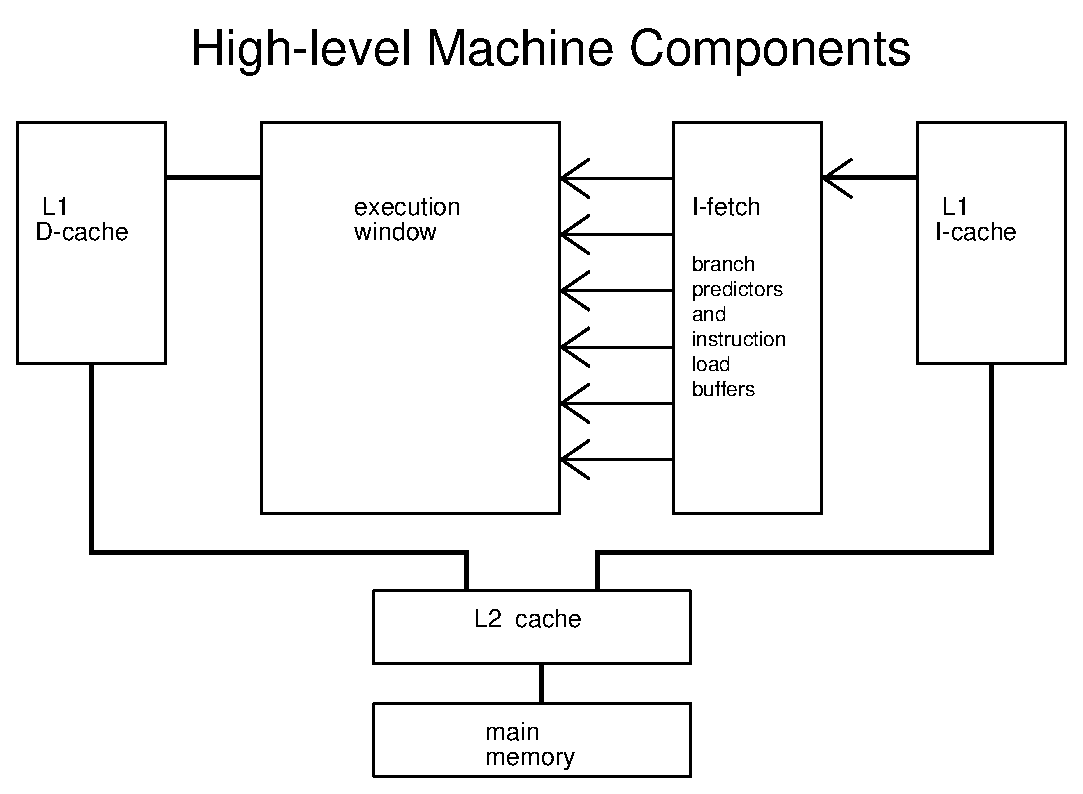
\epsfig{file=high.eps,width=4.0in}
\caption{{\em High-level View of the Distributed Microarchitecture.} 
Shown are the major hardware components of the microarchitecture.
With the exception of the 
execution window block, this is similar to most conventional
microarchitectures}.
\label{fig:high}
\end{figure}
%
At the level of detail shown in Figure \ref{fig:high}, this
microarchitecture is fairly similar to most conventional
microarchitectures.
The main memory block (usually the system DRAM),
the L2 cache (unified in the present case), and the L1 instruction 
cache are all the same as what is commonly used today in exiting
machines.
Except for the fact that the main-memory, L2 cache, and L1 data
cache are all address-interleaved, there is nothing further
unique about these components.  Our L1 instruction
cache is presently not address-interleaved.
The interleaving of memory based on address basically provides an easy way
to substantially increase the bandwidth throughout the
memory system.  This is a common technique for increasing
memory bandwidth that has already been used extensively
and continues to be so.
The component labeled \textit{execution window} is where
our microarchitecture differs substantially from existing machines.
This component is discussed in more detail later.

Although our L1 data cache appears similar (at this level) to 
a convention data cache, it has a special feature within it
that is used to track speculative memory writes.
We allow speculative memory writes to propagate
out to the L1 data cache.  Multiple copies
of speculative writes may be present within the L1 data cache
at the time time.  The are differentiated from each other
through the use of time-tags.  Time-tags are the basic mechanism
used in the microarchitecture to order all operands including
memory operands while they are being used by instructions
currently in-flight.
More information on both the L1 data cache and the whole of
the memory subsystem in general is given in a report
by Uht \cite{Uht02b}.

The i-fetch unit first fetches instructions from i-cache
along one or more predicted program paths.
In our microarchitecture, instructions are immediately
decoded after being fetched.
All further handling of the instructions is done in their decoded
form.
The primary function is to stage decoded instructions 
into a \textit{load buffer}
so that they are available to be shifted into the execution
window.  This load buffer is organized so that
a large number of instructions can be broadside loaded into the
execution window in a single clock.
The multiple buses going from the i-fetch unit to the
execution window in Figure \ref{fig:high} is meant to
reflect this operation.  Six buses are shown in that figure
and the significance of that number will shown in the
section that discusses the execution window.
The number of instructions that can be loaded simultaneously
in a single clock will be later referred to as 
the \textit{column height} of the machine.  This meaning
of this will become
evident in the section discussing the execution window.

The execution window component 
represents the major departure of our microarchitecture
from all previous and existing ones.
Calling this part of the machine a component is actually somewhat
misleading since it is the majority of the hardware resources
for the whole of the microarchitecture (as will become quite evident).
The execution window will contain all of the instructions
that are in flight within the actively being executed.  This may be an
exceedingly large number as compared with 
existing conventional microarchitectures.
Due to the size and complexity of the execution window, it is
discussed in much more detail in the next section.
%
\subsection{The Execution Window}
%
Instructions within the execution window may be both actively 
executing
or may be waiting to be re-executed when events indicate that
a re-execution is warranted or required for proper program order
fulfillment.
Figure \ref{fig:window} shows a more detailed look
at the execution window.
This view is still at something of a high level but serves to
illustrate the main subcomponents with it.
The i-fetch unit is shown again on the far right as a reference.
%
\begin{figure}
%\vspace{0.2 in}
%\setlength{\epsfxsize}{10cm}%7
%\centerline{\epsfbox{window.eps}}
\centering
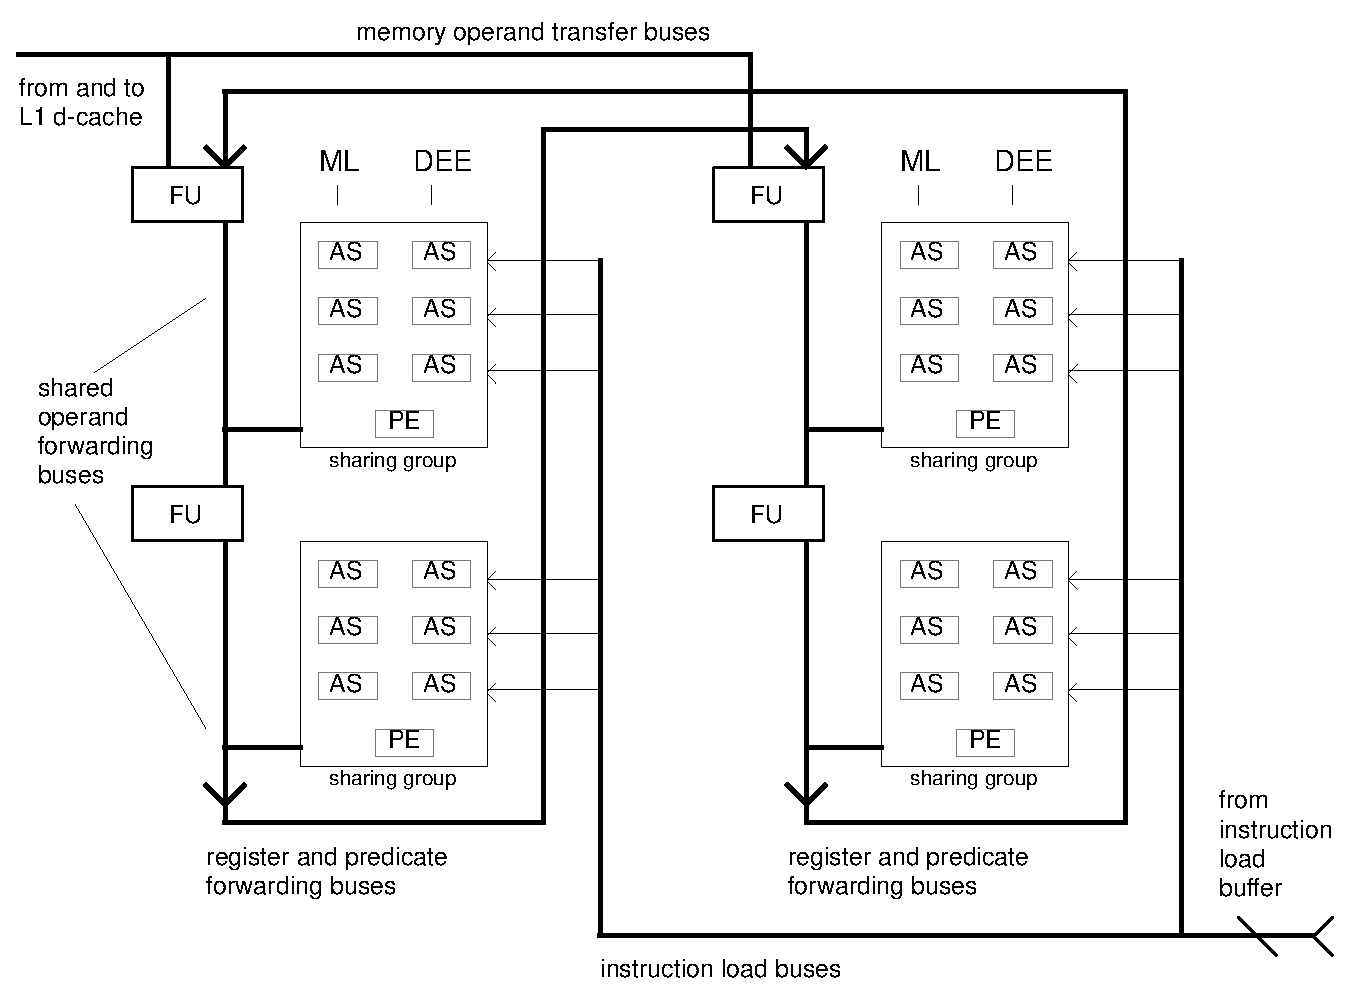
\epsfig{file=window.eps,width=5.8in}
\caption{{\em High-level View of the Distributed Microarchitecture.} 
Shown is a layout of the Active Stations (AS) and Processing Elements (PE)
along with some bus interconnections to implement a large,
distributed microarchitecture.}
\label{fig:window}
\end{figure}

We have extended the idea of Tomasulo's reservation
station \cite{Tom67} to provide the basic building block for a distributed
microarchitecture.  Tomasulo's reservation station provided for the
simultaneous execution of different instructions over several
functional units.  
Register results from the functional units were placed on
a common data bus and looped back to provide source register operands 
for instructions waiting in the reservations stations as well as
for updating of the register file.  In our microarchitecture,
output results are not looped back to the inputs of the reservation
stations
that provided the results but are rather forwarded to a new set of
stations that form a new spatially separate group from the first.  
We
also extend the idea of the reservation station to allow for multiple
executions (re-executions) of the same instruction in the station.  We
keep instructions in their associated stations station until they are
retired (either committed or squashed).  We call our adaptation of the
reservation station the \textit{active station} (\textit{AS}).

Rather than lay the active stations out in silicon simply next to
function units that will execute the instructions loaded to them
(like with the original reservation station idea),
we lay them out in a two dimensional grid whereby sequentially
loaded instructions will go to sequential ASes down a column of
the two dimensional grid of ASes. 
The number of ASes in the height dimension is referred to
as the column height of the machine, which was introduced
previously.
Figure \ref{fig:high} therefor showed a column height of six.
The column height can be seen more clearly in 
Figure \ref{fig:window} also when one counts the total
number of ASes that form a given column of ASes.

Dispersed among the active stations are associated execution
units.  These executions units are represented in the figure as
a \textit{processing element} (\textit{PE}).  
Although an AS always only holds at most a single instruction,
PEs may consist of a unified all-purpose execution unit capable of
executing any of the possible machine instructions or
several functionally partitioned units individually tailored
for specific classes of instructions (integer ALU, FP, or other).

Groups of active stations along with their associated processing
element
are termed \textit{sharing groups}.  Sharing groups somewhat resemble
the relationship between the register file, reorder buffer,
reservation stations, and function units of most conventional
microarchitectures.  They have a relatively high degree of bus
interconnectivity between them as conventional microarchitectures do.
In our case, the active stations serve the role of both the
reservation station and the reorder buffer of more conventional
machines.

Referencing again the example machine layout
of Figure \ref{fig:window}, it can be seen that the machine
shown consists of 
two columns of sharing groups.  
Each sharing group contains two columns of
active stations (the specific use of which is explained later).
Each sharing group also contains three rows of active stations
and a single processing element in the shown case.  
Of course, most machines capable of substantial ILP
speedups require larger, or much larger, numbers of
components than shown in this example.
Typical machine configurations explored so far have been in the
range of having eight or more sharing groups per column, each
with as many as sixteen or more active station rows per sharing
group.  Additionally, typical machines have as many as eight to
32 or more columns of sharing groups.
We generally characterize
a basic machine configuration according to the tripple: 
%
\begin{itemize}
\item{sharing group rows}
\item{active station rows per sharing group}
\item{sharing group columns}
\end{itemize}   
%
These three characteristic parameters of a given machine
are greatly influential to the performance of the machine
and therefor form a basic configuration on which experiments
are performed to explore other aspects of the machine.
We often refer to these three parameters as the \textit{geometry} 
of a given machine.
We normally
show these above three numbers concatenated with 
a hyphen so that the machine shown
in the figure, as an example, would be abbreviated {\tt 2-3-2}.
When a maximum number of alternative speculative execution
paths is being explored (employing multipath execution), 
the number of alternative speculative paths is often added
with an additional number to the above abbreviation.
For the shown machine in the figure with a maximum number 
of alternative paths 2 (for example), providing for a total
of 3 speculative execution paths, the abbreviation for it 
would be {\tt 2-3-2-2}.

The less bold horizontal buses (referencing Figure \ref{fig:window})
form the paths by which instructions are loaded to active stations
from the decoded instruction load buffers discussed previously.
These buses are unidirectional and can be, and typically are,
buffered at desired spatial intervals to provide 
scalability in the horizontal dimension
of the execution window.
Again, the instruction fetch unit is responsible for
fetching instructions from the memory hierarchy, these are then decoded
and placed into the load buffers.   

Also employed within the execution window is a scheme to
dynamically predicate, at execution time, 
all instructions that have been loaded
into active stations.  
This predication scheme essentially provides for each loaded instruction
an \textit{execution predicate}.  These execution predicates
are just a single bit (like with explicit architectural predication)
but are maintained and calculated within the microarchitecture
itself and are thus not visible at the ISA level of abstraction.
A full discussion of the execution-time predication scheme
is beyond the scope of this present paper.

The following subsections further describe some subcomponents
within the execution window.
There are many possible options for implementing many
of the subcomponents required.
Many variations of these subcomponents and their interconnections
have already been explored but a subset of these is
presented in this present work.
%
\subsubsection{Interconnection Fabric and Machine Scalability}
%
A scalable interconnect fabric 
is provided to forward result
operands from earlier active stations to later active stations in
program order.  Result operands consist of register, memory, and
instruction execution predicates (as briefly discussed above).  
The interconnect fabric is simply shown by
the bold (primarily vertical) buses in 
Figure \ref{fig:window}.
There is not necessarily one type of interconnection
fabric possible for the forwarding of operands (of any of the
three types)
and we have explored several
different types and methods of operand forwarding already.
Each operand forwarding bus can actually consist of several
buses in parallel.  This is indicated by the use of the
bold lines to depict the buses.  The use of more than one
bus in parallel has generally been required to meet
the bandwidth needs of the machine.

In this paper, we present just two of several methods that
may be possible for the forwarding of any of the three types of
operands (register, predicate, and memory).
We use one method for the forwarding of register and predicate
operands and a second method for the forwarding of memory 
operands.
Each of these has a different type of interconnection fabric
associated with it.
The two types of interconnect fabric used 
in our present microarchitecture
can be discerned
in Figure \ref{fig:window}.
The set of interconnection buses used for register and predicate
operand forwarding are labeled near the top of the 
figure \textit{register/predicate forwarding buses}.
The interconnection buses used for memory operand forwarding
are labeled \textit{memory operand broadcast buses}.
All types of interconnection fabrics employ active repeater
components of one sort or another within them.
These active repeater components are
used (and required) to maintain constant bus lengths
(wire spans) needed for scalability.
The active repeater components for the register and
predicate forwarding are termed 
the \textit{register filter unit} (RFU)
and the \textit{predicate forwarding unit} (PFU)
respectively.  
These are shown combined in the figure
labeled as \textit{R/P FU}.
The active repeater component used for the memory
operand forwarding fabric is termed a \textit{memory filter unit} (MFU)
and is labeled as such.
Register and predicate operand forwarding can
use separate bus resources (and we have explored that previously) but
for the present work described, we have used a scheme where
they share common buses to perform their forwarding operations.
These units do more than just repeat operand values from
one span of a bus to the next (as their names suggest).
The RFU and MFU have the ability to try to
to \textit{filter} unnecessary forwarding operations from
occurring.  This is a means to try and reduce the overall bandwidth
requirements of the forwarding interconnection fabric.
The MFU is also frequently termed a \textit{L0 data cache}
since it indeed effectively has a cache of speculative
memory values stored within it.

As can be seen 
in Figure \ref{fig:window},
the register and predicate operand forwarding buses
loop around from the bottom of left adjoining columns to the tops of
the right adjoining columns.  The forwarding from the far lower right
also loops around to the far upper left.  In all, the register and
predicate forwarding
buses (their interconnection fabric) form the characteristic ring pattern,
inherent in many microarchitectures.
They pass by each sharing group in the execution window providing
forwarding access for them.
For our register and predicate forwarding buses
used in the present work, we employ several buses in parallel.
Requests for bus use will be satisfied with any bus slot that may be
available on any of the buses in parallel, belonging to
a given span.
Optionally, a particular forwarding bus could be selected
for a given forwarding operation based on the address of the
architected register itself, but this has not been explored further.
The work presented in this paper uses four parallel buses
for the register and predicate forwarding requirements.
Other numbers of parallel buses have been explored but that
work is not elaborated further in this present paper.
As mentioned previously, RFUs form the active repeater
component for the forwarding of register operands,
and PFUs serve the same purpose for predicate operands.
The present diagram shows all of the individual buses in 
a span being repeated together at designated span intervals.
This is not necessarily required.  Rather, individual buses, that may
make up a parallel bundle of buses, do not have to start and
terminate at the same repeater unit.
Although staggered repeating of individual buses has been
explored, only the case of repeating all of the buses
making up a bus bundle is presented in this paper.

In contrast to the register and predicate operand forwarding 
interconnection fabric,
the memory forwarding fabric in this present work employs
a two-staged star-like topology rather than a serpentine
loop-around topology.
From 
Figure \ref{fig:window}, it can be seen that
the hub of the star is at the top
of the machine and is the bus span that is indicated as
connecting to the L1 data cache (not shown) on the left of
the figure.  This horizontal portion of the interconnection
scheme may be further broken up into smaller spans by
active repeater elements but these are not shown in the present
diagram.  Memory Filter Units (MFUs) are shown coupling the
top horizontal bus span to the the vertical spans that
go down each column of ASes.  Each vertical span can be
further subdivided by MFUs in order to keep each bus span
at a constant spatial length (constant wire lengths) as
well as having a constant number of logic loads as the machine
scales in the vertical dimension.
There are always MFUs present to couple the vertical portion
of the fabric to the horizontal portion.
Like the register and predicate forwarding buses,
several buses may be used in parallel to increase the
forwarding bandwidth for each span.
Unlike the register and predicate buses, the individual
buses used for memory are generally differentiated
by being address-interleaved.  That is, a specific bus
is chosen (arbitrated for) to forward a particular memory
value based on the address of the value being forwarded.
This makes for simpler arbitration logic than that which
is need for the arbitration for register and predicate buses.
%
%
\subsection{Basic Machine Operation}
%
Instructions are fetched from memory, decoded, and staged in 
load buffers.
When an entire column
of active stations is free to accept new instructions, generally
an entire column of instructions are loaded to the free active station
column from the load buffer.  Partial column loads are possible
also but represent a loss of resource efficiency.
Conditional branches are
predicted at or just before they are entered into the load buffers
(for subsequent load to the ASes).
The prediction of the branch outcome 
prediction is sent along with the
decoded instruction information when instructions are 
loaded to ASes.

All of the active stations in a given column are loaded with 
instructions in a single clock.  
In our present implementation, newly loaded instructions
are only loaded to a single column of active stations within
a column of sharing groups.  The other column of active stations
in our current sharing groups (which currently have a total
of two columns of ASes) is reserved for the spawning of additional
execution paths as a result of a condition branch instruction.
When and how additional paths are spawned is discussed later.

It should be noted that there are several strategies for
loading instructions to available active station columns.
Since all loaded instructions are speculative, instructions
from either outgoing path of a conditional branch can be loaded
to sequential active stations.
The fetch unit is responsible for preparing for such decisions.
Even when a conditional branch is predicted as being taken,
instructions may still be loaded sequentially down the not-taken
path under most circumstances.  If the distance to the target 
of a branch
that is predicted to be taken is not too large,
instructions may be loaded along the program static order (or not-taken
path) of the branch in the hopes of capturing hammock styled branch
constructs.  A more detailed discussion on these alternatives is
presented later in the paper.

Program dependencies (control, register, and memory) are 
maintained through the use of time-tags that
are associated with all forwarded operands.
This has some resemblance to register tags used in more conventional 
microarchitectures but has been more generalized for use in this
distributed microarchitecture.  Instructions remain in their
associated active stations until they are retired by either being
committed or abandoned (squashed).  In this way, the active stations
(or rather the whole set of them)
fulfill the role of the reorder buffer or register update unit of more
conventional microarchitectures.

Much more detailed information about this microarchitecture
can be found in a technical report by Uht et al~\cite{Uht01}.
Additionally, a more detailed discussion of the mechanism used for
enforcing program dependencies in this microarchitecture
can be found in a report by Kaeli et al~\cite{Kaeli01}.
A more detailed discussion about multipath execution and
the spawning of alternative speculative execution paths is given
in the following section.
%
%
\subsection{Conditional Branches and Multipath Execution}
%
The run-time machine microarchitecture only has limited information
available to it for making certain optional decisions.
There are two major alternatives that the machine needs to constantly
consider.  The first is whether to load instructions to sequential
ASes following
the not-taken path of the condition branch or to load instructions
along the taken path.  
The second major decision to make is
whether to spawn an alternative speculative path
on any given conditional branch.
The machine only has the following information
available at run-time for making microarchitectural decisions :
%
\begin{itemize}
\item{distance to the target of the branch -- near/far}
\item{branch target direction -- forward/backward}
\item{the branch outcome prediction}
\end{itemize}   
%
Branches with \textit{near} targets are those where
the distance from the branch to the target is smaller than
the total number of instructions that the machine can have
in-flight simultaneously.  All other branch targets are considered
\textit{far} targets.

First, if a backward branch is predicted taken,
we will speculatively follow it and continue loading instructions
into the execution window for the mainline path from the target
of the branch.  
For a backward branch that
is predicted not-taken, we continue loading following the
not-taken output path.

If a forward branch has a near target (small domain size), then we
load instructions from the domain of the branch (following the
not-taken output path) whether or not it is the most predicted path.
Our mainline path continues along the predicted branch output path
regardless of whether it was the taken or not-taken one.  
We spawn a disjoint
alternative path for the opposite output of the branch from
the mainline path case, whatever it is.
This action
provides the benefit of having both the domain and target of the branch
in the execution instruction window of the machine.  

For forward branches with a far target,
if the branch is predicted taken, we load instructions following the target
of the branch.  If the branch is predicted not-taken, we continue
loading instructions for the mainline path following the not-taken
outcome of the branch.  In both of these cases, we do not
spawn an alternative path for this branch.
%
%
%
\section{Simulation Results}
%
We present results from simulations of a set of machine configurations
using the general microarchitecture described previously.
We first describe something about our simulation process.
We present the IPC results for three studies done on the simulated
microarchitecture.

The first study explores the effects of multipath execution
on machine performance (as measured by the resulting IPCs
for our benchmark programs).  In this first study, five
basic machine configurations are explored across all of our
benchmarks.  We first
provide results the the case when no alternative speculative paths are used
(the machine is executing in single-path mode only).
We then present results using one of two possible
strategies for managing additional speculative execution paths.
Then we present results using a different strategy for managing
the multipath execution.

In our second study, we explore the effects of varying
memory system parameters (access latencies) on a fixed sized configuration
of the machine.
This study serves to show how sensitive the microarchitecture
is when some variability of performance is present in individual
memory system components.

In our third study, we present some data showing
the sensitivity of the microarchitecture to a varying parameter
of the second strategy for
the management of multipath execution.
This is an attempt to evaluate this particular strategy for its maximum
effectiveness as it affects ultimate program performance.
%
\subsection{Methodology}
%
The simulator is a recently built tool that shares some similarity
to SimpleScalar \cite{Austin97} but which was not based on it.
We execute
SpecInt-2000 and SpecInt-95 programs on a simulated machine
that features a MIPS-1 ISA along with the addition of some MIPS-2 and
MIPS-3 ISA instructions.  We are using the standard SGI Irix system
libraries so we needed to also support the execution of some
MIPS-2 and MIPS-3 instructions to accommodate
that.  All programs were compiled on an SGI machine under the
Irix 6.4 OS and using the standard SGI compiler and linker.  
All benchmark programs were compiled with
standard optimization ({\tt -O}) for primarily the MIPS-1 ISA ({\tt -o32}).
No changes to the SGI compiler or linker were made to create
the binary benchmark programs.

For our benchmark programs, we chose five programs to work with.
We chose four programs from the SpecInt-2000 benchmark suite
and one program from the SpecInt-95 program suite.
The benchmark programs explored along with some statistics 
are given in Table \ref{tab:benches}.
All program were executed using the SpecInt reference inputs.
All accumulated data was gathered over the simulated execution of
500 million instructions,
after having skipped the first 100 million instructions.
The first 100 million instructions, however, were used to warm up the
various simulator memory caches.
%
\begin{table}
\begin{center}
\caption{Benchmarks Programs Simulated and Some Statistics.}
\label{tab:benches}
\begin{tabular}{|c|c|c|c|c|}
\hline 
benchmark&
br. prediction accuracy&
avg. L1 miss rate&
dynamic cond. brs.&
forward brs.\\
\hline
\hline 
bzip&90.5\%&98.5\%&7.0\%&81\%\\
\hline 
parser&92.6\%&98.3\%&13.0\%&85\%\\
\hline 
go&72.1\%&96.6\%&9.0\%&89\%\\
\hline 
gzip&85.4\%&97.0\%&8.8\%&85\%\\
\hline 
gap&94.5\%&98.9\%&6.2\%&91\%\\
\hline
\end{tabular}
\end{center}
\end{table}
%
\subsection{IPC Results for Singlepath and Multipath Execution}
%
In this section, we present IPC data over six major configurations
of the machine.  We have results for three different cases
for multipath execution.  These are : no multipath execution (singlepath),
simple multipath execution , and enhanced multipath execution.

We will first present IPC data for the benchmarks running
with only singlepath speculative execution.  In this case, no
alternative speculative paths are spawned when conditional
branches are encountered.
We next present the IPC data for the same benchmarks running
on the same machine configurations when a simple
strategy for spawning disjoint paths is used.
In this simple strategy, we will spawn disjoint paths for conditional
branches on a first come, first served basis.  That is, as machine
execution resources become available for the speculative execution
of a disjoint path, those resources are assigned to the next conditional
branch for which an alternative speculative path has not already 
been assigned.  The alternative speculative path is allowed to
remain executing until its associated originating conditional
branch get resolved (at which point its alternative speculative
path is squashed).
Thirdly, we present IPC data for the same machine configurations
but now using a slightly more sophisticated strategy for the management
of alternative speculative disjoint paths.
With this strategy, 
disjoint paths are again assigned to the next already unassigned
conditional branch as before but now when a conditional branch
has had a disjoint path resident within the execution window for a certain
minimum amount of time,
its associated alternative speculative path
is squashed (or as we often say, it was released) in order to make room for
the spawning of additional alternative speculative paths.
We term this the \textit{release} strategy of managing
alternative speculative paths.
The rational is that as a conditional branch gets closer to
being resolved, the likelihood of it being mispredicted becomes
less and approaches zero.  When a conditional branch is resolved,
its likelihood of being further mispredicted is, by definition,
zero.  We attempt to take advantage of this to free up execution
resources associated with these branches and assign them to the
next unassigned conditional branches.

The numbers of each of the major machine components, for each of the six
simulated configurations, are given in Table \ref{tab:configs}.
Although we have explored a large number of various sized
machines, these particular configurations were chosen in order
to get a range of IPC performance across a number of very
different machine sizes and shapes (geometries).
The common machine characteristics used in this section for
obtaining IPC results is given in Table \ref{tab:params}.
These machine characteristics are fairly representative of
existing typical values.  Our choice for the main memory
access latency is substantially conservative for an existing
1 GHz machine but might be more typical of a 4 or 5 GHz machine
a few years from now.  Main memory performance is dominated
by DRAM technology and major improvements in speed are not soon
expected over the current fastest devices \cite{Sam99}.
%
\begin{table}
\begin{center}
\caption{Machine configurations simulated for each of the benchmark
programs.}
\label{tab:configs}
\begin{tabular}{|c|c|c|c|}
\hline 
SG rows&
ASes per SG&
SG columns&
max D-paths\\
\hline
\hline 
8&4&8&8\\
\hline 
32&2&16&16\\
\hline 
32&8&16&16\\
\hline 
8&8&8&8\\
\hline 
16&8&8&8\\
\hline
\end{tabular}
\end{center}
\end{table}
%
\begin{table}
\begin{center}
\caption{General machine characteristics.}
\label{tab:params}
\begin{tabular}{|l|l|}
\hline 
L1 I/D cache access latency&1 clock\\
\hline
L1 I/D cache size&64 KBytes\\
\hline
L1 I/D block size&32 bytes\\
\hline
L1 I/D organization&2-way set associative\\
\hline
L2 cache access latency&10 clocks\\
\hline
L2 cache size&2 MBytes\\
\hline
L2 block size&32 bytes\\
\hline
L2 organization&direct mapped\\
\hline
main memory access latency&100 clocks\\
\hline
memory interleave factor&4\\
\hline
RFU minimum forwarding latency&1 clock\\
\hline
PFU minimum forwarding latency&1 clock\\
\hline
MFU minimum forwarding latency&1 clock\\
\hline
forwarding-bus latency&1 clock\\
\hline
number of forwarding buses in parallel&4\\
\hline
\end{tabular}
\end{center}
\end{table}
%
Table \ref{tab:ipc1} gives singlepath IPC results for each of the benchmark
programs over various machine configurations.
Table \ref{tab:ipc2} gives the results using the simple method for
the spawning of alternative speculative paths.
And Table \ref{tab:ipc3} gives the results using the \textit{release} 
method for
the spawning of alternative speculative paths.
The configuration labels 
(4-tuples) 
at the tops of these tables consist of the concatenated 
numbers of
machines components for: SG rows, AS rows per SG, SG columns,
and the maximum DEE paths allowed for that execution.
In addition to the individual benchmark IPC results, we also
present the harmonic mean of the IPC across all benchmarks.
For the last data set, disjoint paths were released when their
associated conditional branch came
within XX sharing group columns of being resolved (committed).
That is, when the machine executes to a point where a conditional branch
with an associated disjoint path gets to be the XX sharing group column
from being next committed, its associated disjoint path is released.
%
\begin{table}
\begin{center}
\caption{IPC results for singlepath execution.}
\label{tab:ipc1}
\begin{tabular}{|c|c|c|c|c|c|}
\hline 
configuration&
8-4-8-8&
8-8-8-8&
16-8-8-8&
32-2-16-16&
32-4-16-16\\
\hline 
\hline
bzip2&3.4&4.2&4.8&4.2&4.7\\
\hline 
parser&2.9&3.3&3.8&3.5&3.9\\
\hline 
go&2.6&3.2&3.7&3.4&3.6\\
\hline 
gzip&3.4&4.4&5.2&4.8&5.3\\
\hline 
gap&4.5&5.6&6.1&6.5&6.3\\
\hline
\hline 
HAR-MEAN&3.2&4.0&4.6&4.2&5.6\\
\hline
\end{tabular}
\end{center}
\end{table}
%
\begin{table}
\begin{center}
\caption{IPC results for simple multipath execution.}
\label{tab:ipc2}
\begin{tabular}{|c|c|c|c|c|c|}
\hline 
configuration&
8-4-8-8&
8-8-8-8&
16-8-8-8&
32-2-16-16&
32-4-16-16\\
\hline 
\hline 
bzip2&3.9&4.8&5.5&4.9&5.3\\
\hline 
parser&4.0&4.3&5.1&5.6&5.1\\
\hline 
go&4.6&5.6&6.4&6.0&6.3\\
\hline 
gzip&4.7&5.9&6.8&6.2&6.8\\
\hline 
gap&5.6&6.9&7.1&8.3&7.2\\
\hline 
\hline 
HAR-MEAN&4.5&5.4&6.1&5.8&6.1\\
\hline
\end{tabular}
\end{center}
\end{table}
%
\begin{table}
\begin{center}
\caption{IPC results for multipath execution using D-path release.}
\label{tab:ipc3}
\begin{tabular}{|c|c|c|c|c|c|}
\hline 
configuration&
8-4-8-8&
8-8-8-8&
16-8-8-8&
32-2-16-16&
32-4-16-16\\
\hline 
\hline
bzip2&4.2&5.0&5.8&5.4&5.7\\
\hline 
parser&4.3&4.6&5.3&5.0&5.4\\
\hline 
go&5.1&5.9&6.7&6.5&6.8\\
\hline 
gzip&5.0&6.3&7.0&6.7&7.2\\
\hline 
gap&6.0&7.5&7.5&8.9&7.9\\
\hline 
\hline 
HAR-MEAN&4.8&5.4&6.4&6.2&6.5\\
\hline
\end{tabular}
\end{center}
\end{table}

%
Examining the data, we can see that our simple 
(first-come-first-serve)
multipath execution
strategy significantly outperforms singlepath execution.
This was expected as our microarchitecture is able to
capture many conditional branch domains inside the execution
window and speculatively execute both outcomes of these branches
as a bet against a misprediction.
Our slightly more complicated DEE path \textit{release} strategy
performs better than our simple strategy for all machine
geometry configurations explored here.
%
\subsection{Memory Sensitivity Results}
%
In this section we present IPC data corresponding to varying some
parameters associated with the memory subsystem.
We show IPC speedup results for varying the access latencies,
in clocks, for: L1 I-cache,
L1 D-cache,
L2 cache, and
main memory.
All of this data was gathered on a machine geometry configuration
of 16-8-8-8 with the other parameters (the ones that are
not varied) being those that are listed in Table \ref{tab:params}.
Figure \ref{fig:mem1} presents the speedups for varying
the L1 I-cache hit latency clocks from zero through eight.
Figure \ref{fig:mem2} presents IPC speedup results
as the L1 D-cache hit latency is varied from zero clocks through to
eight clocks.
Figure \ref{fig:mem3} presents the speedup results
as the L2 cache (unified I/D) hit latency is varied from 
zero clocks through to eight clocks.
Finally Figure \ref{fig:mem4} presents the IPC speedup results
as the main memory access hit latency is varied from twenty clocks 
through to 400 clocks.
All IPC speedups in these figures are relative to the zero
access latency cases.  The cases that have zero access latencies
still incur the various bus and active repeater delays that
are inside the execution window of the microarchitecture.
%
\begin{figure}
%\vspace{0.2 in}
%\setlength{\epsfxsize}{14cm}%7
%\centerline{\epsfbox{mem1.eps}}
\centering
\epsfig{file=mem1.eps,width=4.0in}
\caption{Machine IPC speedup results for varying 
L1 I-cache hit delay in clocks.}
\label{fig:mem1}
\end{figure}
%
\begin{figure}
%\vspace{0.2 in}
%\setlength{\epsfxsize}{14cm}%7
%\centerline{\epsfbox{mem2.eps}}
\centering
\epsfig{file=mem2.eps,width=4.0in}
\caption{Machine IPC speedup results for varying 
L1 D-cache hit delay in clocks.}
\label{fig:mem2}
\end{figure}
%
\begin{figure}
%\vspace{0.2 in}
%\setlength{\epsfxsize}{14cm}%7
%\centerline{\epsfbox{mem3.eps}}
\centering
\epsfig{file=mem3.eps,width=4.0in}
\caption{Machine IPC speedup results for varying 
L2 cache hit delay in clocks.}
\label{fig:mem3}
\end{figure}
%
\begin{figure}
%\vspace{0.2 in}
%\setlength{\epsfxsize}{14cm}%7
%\centerline{\epsfbox{mem4.eps}}
\centering
\epsfig{file=mem4.eps,width=4.0in}
\caption{Machine IPC speedup results for varying 
main memory access latency in clocks.}
\label{fig:mem4}
\end{figure}
%
As can be seen from Figures \ref{fig:mem1} and \ref{fig:mem2},
the machine slightly more sensitive to L1 D-cache latency
than to L1 I-cache latency.  This is expected due to the
speculative variability that is present for data memory accesses
that are not likely to present in the instruction accesses.
The GAP program appears less sensitive to L1 instruction or
data latencies and this is probably due to its looping
behavior that provides better spatial and temporal locality
for memory accesses.  Fortunately, latencies of 1 or 2 clocks
for L1 caches is more likely to scale better with increasing
processor clock than memory components further from the processor.

For the L2 cache (ours is currently unified), speedups are
possible for shorter latencies than our present 10 clocks.
Although L2 latencies are likely to also scale somewhat
with future increasing processor clock rates, they are not like
to get scale as well as L1 is expected to do.
Fortunately out machine already gets good IPC performance
at the L2 cache latency of 10 clocks.

With respect to main memory (DRAM), the microarchitecture
is quite insensitive to latencies out to 100 clocks and
only then starts to degrade significantly.  Since 100 clocks
(as we count it -- after our repeater and other bus delays)
is somewhat conservative at the present time (assuming a 2 GHz
CPU clock rate and the latest DDR-SDRAMs), our memory system
arrangement is properly hiding most long DRAM latency as is
generally required.
%
\subsection{Release Strategy Sensitivity Results}
%
In this section we present data corresponding to varying the
parameter used in the microarchitecture that determines when
a disjoint path is \textit{released}.
The parameter that determines when a disjoint path is
released is associated with how long it has been within
the execution window.  
The idea in this strategy is to release disjoint paths
that have been resident for a relatively long period of time
and reassign those execution resources to another (newly spawned)
conditional branch not yet assigned a disjoint speculative path.
We want to explore whether this strategy
is beneficial or possibly detrimental as compared with the
simple disjoint management strategy.
Figure \ref{fig:release} shows the resulting speedups,
as compared with the simple disjoint path management strategy,
as the number of sharing group columns that the conditional
branch for which a DEE path has been spawned has been resident in
the execution window.
Again, this data was gathered on a machine geometry configuration
of 16-8-8-8 with the machine characteristics from
Table \ref{tab:params}.
%
\begin{figure}
%\vspace{0.2 in}
%\setlength{\epsfxsize}{14cm}%7
%\centerline{\epsfbox{release.eps}}
\centering
\epsfig{file=release.eps,width=4.0in}
\caption{Machine IPC speedup results for varying 
release column numbers.}
\label{fig:release}
\end{figure}
%
For this particular machine size (geometry), this strategy
performs worse than the simple strategy when the disjoint
path is released (abandoned) when having been resident in the 
execution window for approximately fewer than 4 or five sharing
group columns.  However, when disjoint paths are retained in the
execution window for approximately
six sharing group columns before their resources are re-assigned,
a performance speedup of about two to five percent is realized.
Several other strategies for the management of disjoint paths
are possible and exploration into some of them will continue.
%
\section{Conclusions}
%
We have presented the overview of a large-scale distributed 
microarchitecture suitable for extracting high ILP from
sequential programs.
This microarchitecture is designed to also implement 
speculative multipath execution.  We presented results
for the machine executing in singlepath mode and two types
of management for paths in multipath mode.
It was shown that multipath execution provides additional IPC
performance over singlepath execution using
both of the heuristics that we explored for
managing disjoint speculative paths.
Further, our enhanced DEE path \textit{release} heuristic provided
an additional average of about five percent better IPC over the
simple DEE path management heuristic for a modest sized machine.
We also showed that our microarchitecture exhibits some
insensitivity to the various memory system component latencies
that are typically encountered in actual designs.
%
\bibliographystyle{latex8}
\bibliography{high}
%
\end{document}
%
%
